\section{Moving Reconstructions}
\label{sec:moving}

\subsection{Purpose}
The TR process assumes that the environment remains fixed between the time-forward and time-reversed steps. It also assumes that the source and target remain fixed between these two steps. However, in a practical WPT system it is desirable to support a receiver in motion. This ability gives a convenience benefit to the consumer, who would not be limited to keeping their mobile device stationary for charging. This is a gap in the current market, which TR may be able to fill. In this section, we propose and investigate a method for using the broad spatial voltage profile to provide a consistent voltage to a receiver in motion.

The experiment is conducted in two parts: mapping the spatial voltage profile of a TR reconstructed signal, and iteratively updating the target location of the time reversal mirror. The first part of the experiment intends to consider the extent to which a reconstruction is localized in space. This property has implications for several parts of the WPT scheme including system efficiency, health concerns, and tolerance in receiver position relative to the target location. A broad reconstruction in space would relate to a lower efficiency, because only a fraction of the energy that is being sent is collected by the receiver. Consequently, if the reconstruction is broad then there is a possibility that some energy could be sent to an unintended nearby medium; for example, the target device might be in a user's pocket, and a a broad profile could indicate that the user themself would be absorbing some of that energy. While both of these effects are generally things that we would like to avoid in a WPT system, it also could facilitate the accommodation of a moving receiver. A profile that is not particularly localized would allow the receiver to shift slightly from the target location and still collect a significant portion of the energy packet that was sent. When the voltage level at the receiver's position drops below some acceptable level, the TR process could be performed again. This would update the target location to the receiver's current location, and reset the voltage at the receiver to the peak value of the reconstruction. A broader reconstruction in space would allow this process to be performed less frequently, while a narrower reconstruction may greatly limit the speed that the receiver could travel at.

\subsection{Spatial Profiling}
\label{sec:spatial-profile}
\subsubsection{Methodology}
The experimental setting for this experiment differs only slightly from that described in section~\ref{fig:ltr-meth}. In this case, the antenna mounted on the scanning panel is designated as the receiving antenna. Motion of the receiving antenna is achieved using an externally-mounted PI MikroMove \texttt{M-415.DG} translation stage and the enclosure remains sealed during the translation. An interrogation pulse is used to create a reconstruction at the middle of the scanning range. The receiver is then stepped through the entire scanning range, at a step size of 0.2 mm. At each position, the peak to peak voltage of the reconstruction is measured and recorded. This experiment is repeated for a variety of frequencies to test for a wavelength dependence.

\subsubsection{Results}
\label{sec:profile-results}

\begin{figure}[t!]
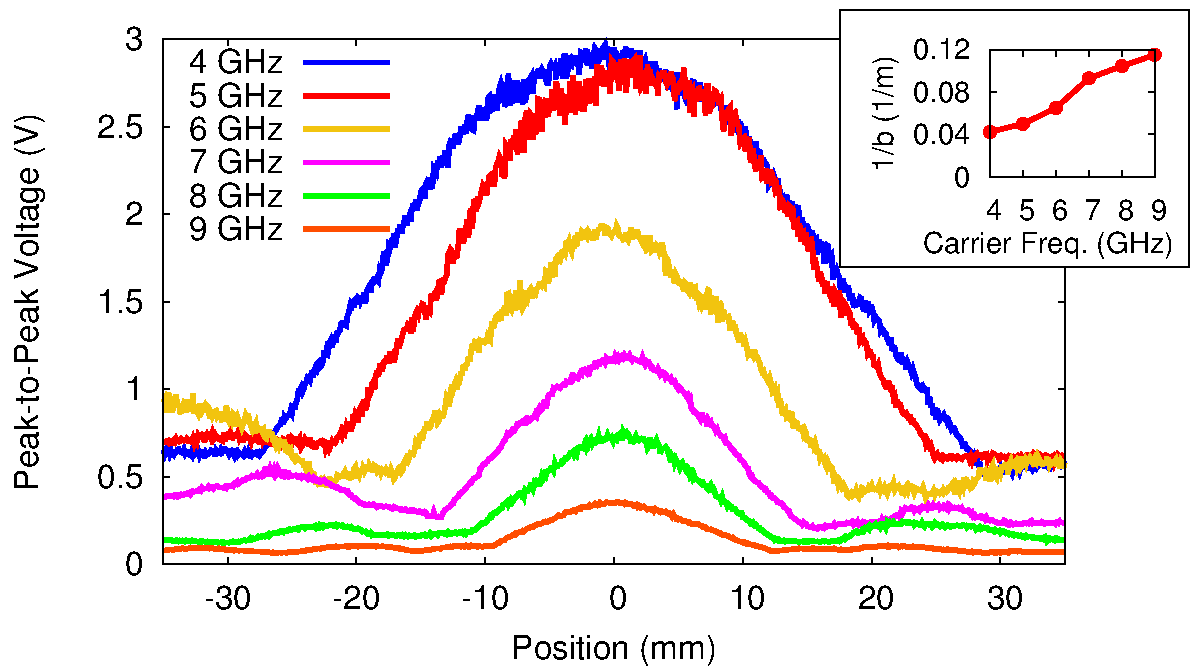
\includegraphics[width=\columnwidth]{spatial/freq_profile.pdf}
\caption{Spatial profile of peak-to-peak voltage amplitudes of reconstructions
investigated at carrier frequencies ranging from 4 to 9 GHz in 1 GHz
steps.  The inset shows the inverse of the fit $b$ values versus carrier frequency, showing the expected linear relationship.}
\label{fig:spatial-freq-profile}
\end{figure}

\begin{figure}[t!]
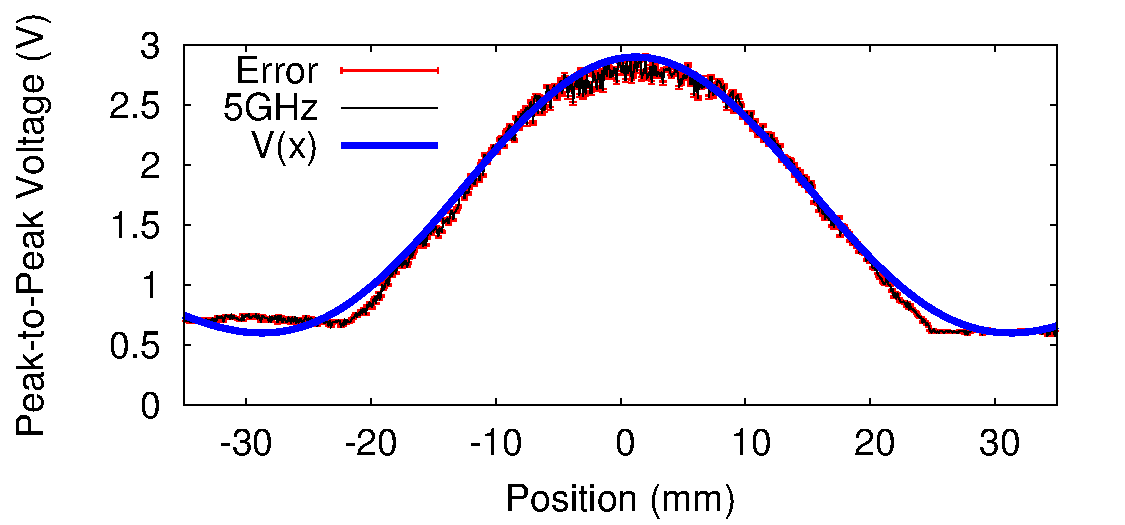
\includegraphics[width=\columnwidth]{spatial/fit.pdf}
\caption{Measured peak-to-peak voltage amplitude of reconstructions received in the
vicinity of a time-reversed wave collapse location with a 5 GHz carrier
frequency, and fit to the \texttt{sinc(x)} function.}
\label{fig:spatial-error-fit}
\end{figure}

The reconstruction peak-to-peak voltage profile is expected to take the form of a $sinc(x)$ function about the target location~\cite{lerosey-focusing}. Thus, the following equation is proposed to predict $V(x)$, the maximum peak to peak voltage from a given reconstruction, as a function of $x$, the distance between the reconstruction focal point and the receiver:

\begin{equation}
\label{eq:vx}
V(x) = a\cdot sinc\left(\frac{x+c}{b}\right) + d
\end{equation}

where $a$ is the maximum peak-to-peak reconstruction amplitude, $b$ is the half-wavelength, $c$ is the location of the antenna along the x-axis, and $d$ is the noise level
offset voltage. Since $b$ is proportional to the wavelength (and inversely proportional
to frequency), as the carrier frequency is increased,  $\frac{1}{b}$ also increases, causing the ``bubble'' of the sinc function in Fig~\ref{fig:spatial-freq-profile} to get smaller. This relationship is shown explicitly in the inset of Figure~\ref{fig:spatial-freq-profile}. Figure~\ref{fig:spatial-error-fit} shows Equation~\ref{eq:vx} fit to the 5 GHz curve from Figure~\ref{fig:spatial-freq-profile}, including error bars. The fit is good, but has a reduced $\chi^2$ of 234 due in part to the rather large background noise level. The error bars are primarily systematic, introduced by the oscilloscope internal voltage multiplier used in scaling.


The results presented in Figure~\ref{fig:spatial-freq-profile} allow us to draw several conclusions. In this frequency range, the reconstructions can be categorized as broad, spanning several centimeters in width. This is a significant conclusion because it indicates that we can move the receiver slightly away from the target location and still collect energy from the reconstruction. This allows us to implement a system targeting a moving receiver as previously described.

\subsection{Reconstructing on a Moving Target}
\label{sec:recon-moving}

\subsubsection{Methodology}
For this experiment, the receiving antenna was moved at a constant speed of 0.2~$\frac{mm}{s}$ across the entire 70~mm range provided by the \texttt{MikroMove}. To counteract the degradation of reconstruction strength as the antenna moved, we periodically repeated the interrogation step, effectively re-centering the reconstruction on the antenna. Since the test equipment does not allow broadcast of one sona while collecting another, it was not possible to transmit power during the collection time, leading to a finite ``dead time'', denoted $t_d$ in Figure~\ref{fig:moving-recon}. During the broadcast period, the time-reversed sona was continually broadcast into the cavity (once every 15~$\mu$s) and the peak-to peak voltage across the receiver was measured once every 2.05~seconds, meaning that the reconstructions are highly undersampled in this plot. After every 15 samples were collected, the process was repeated. We refer to this full process of collecting a new sona and then broadcasting it for a given period time as a full ``cycle'' of length $t_c$. The results in Fig. 6.1 below were obtained using a carrier frequency of 5 GHz, $t_d$ of 7 seconds, and $t_c$ of 39.8 seconds. Based on the results from Section~\ref{sec:spatial-results}, the peak-to-peak reconstruction voltage measured by the receiver is expected to decay according to the $sinc(x)$ function as the receiver
moves away from the reconstruction focal point. This $sinc(x)$ function will be centered on the position where the sona was last collected, making the reconstruction focus continually lag behind the antenna. Consequently, the maximum reconstruction strength is limited by the time needed to collect, time reverse and re-broadcast an updated sona. The following equation is proposed as a model for the peak-to-peak voltage of the reconstruction on a moving target as a
function of time, assuming a constant velocity $\bar{v}$:

\begin{equation}\label{eq:vt}
%\begin{displaymath}
  V(t) = \left\{
        \begin{array}{ll}
                0 & : t\pmod{t_c} \le t_d \\
                a\cdot sinc(\frac{\bar{v}t}{b})+d & : t\pmod{t_c} > t_d
        \end{array}\,.
  \right.
%\end{displaymath}
\end{equation}

\subsubsection{Results}
\label{moving-results}

The results of this experiment are very promising. We hypothesized that the reconstruction peak to peak voltage would reset back to a maximal value when a new sona was used to refocus the reconstruction, and follow the voltage profile as the receiver moved away from the new target location. This was almost exactly confirmed by the experimental results. This is encouraging for the application of TR to a practical WPT scheme because it proves the applicability to a moving receiver system.

\begin{figure}[t]
\centering
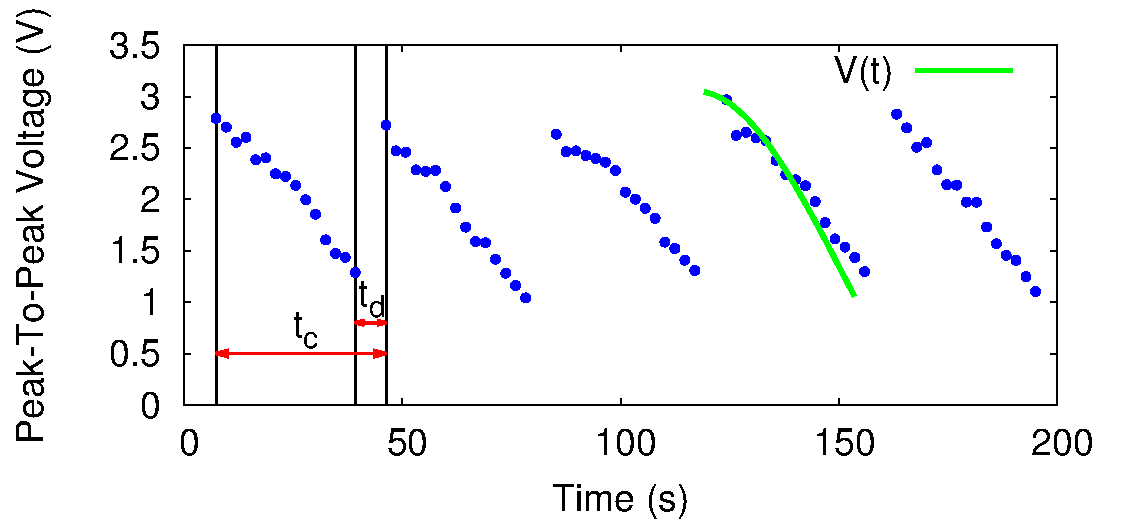
\includegraphics[width=0.85\textwidth]{moving/moving_recon}
    \caption[Voltage measured during moving reconstructions]{Reconstruction voltage amplitude vs. time as the target moves along one wall of the enclosure. A new sona signal is acquired every $t_c = 39.8s$, leading to a dead time of duration $t_d = 7s$. The target is moving at a speed of 0.5~$\frac{mm}{s}$ and the carrier frequency is 5~GHz. The green line is Eq.~ref{eq:vt}.}
    \label{fig:moving-recon}
\end{figure}

It is worth noting that the speed of the receiver is relatively slow at 0.2 millimeters per second. This experiment is intended to be a proof-of-concept, with generalized equipment that carries significant overhead. The GPIB connections between the signal generators, oscilloscope, and workstation contributed to the long delay between system operations, in addition to the slow processing speed of the equipment itself. We expect that with a dedicated time reversal system, the TR process of reacquiring a new target location could be performed in milliseconds instead of seconds. This would greatly increase the maximum receiver speed that could be accommodated. By refocusing the reconstruction more often, the average peak to peak voltage can be raised closer to that maximal value, but the dead time of the system is increased. With further research and engineering work, the possibility of a TR WPT scheme that can power a receiver in motion can certainly be realized. 
